\section{Design of the Chorus and Flanger Effect}

\subsection{Obtaining the Differential Equation}

The flanger- and chorus- effect are similar in their design so they will be presented in the same section. \\

From the block diagram presented in section \autoref{sec:chorus}, a block diagram in the discrete time domain for the flanger and chorus effect can be obtained and is shown in \autoref{fig:chorus_diag_des}. \\ 
The chorus effect is the one in red and black while the flanger is only in black.  
\begin{figure} [htbp!]
	\centering
\begin{picture}(0,0)%
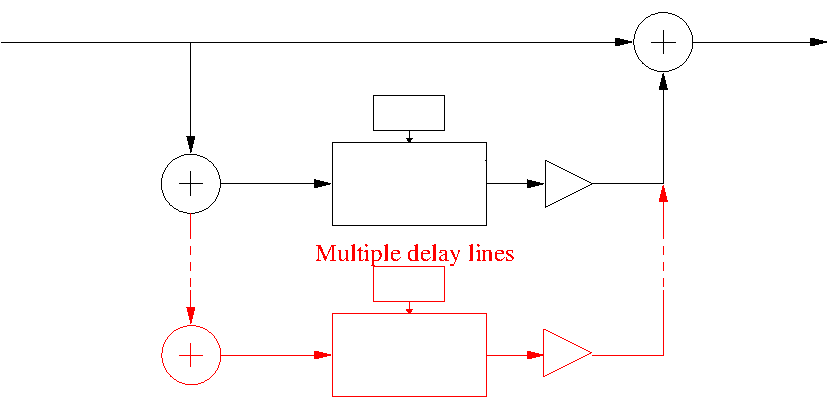
\includegraphics{chorus_diag_des.pdf}%
\end{picture}%
\setlength{\unitlength}{4144sp}%
%
\begingroup\makeatletter\ifx\SetFigFont\undefined%
\gdef\SetFigFont#1#2#3#4#5{%
	\reset@font\fontsize{#1}{#2pt}%
	\fontfamily{#3}\fontseries{#4}\fontshape{#5}%
	\selectfont}%
\fi\endgroup%
\begin{picture}(6327,3018)(3766,-3493)
\put(6571,-1906){\color[rgb]{0,0,0}$z^{-d_{1}}$}%

\put(8101,-1636){\color[rgb]{0,0,0}$g_{1}$}%

\put(6616,-3211){\color[rgb]{1,0,0}$z^{-d_{2}}$}%

\put(8101,-2986){\color[rgb]{1,0,0}$g_{2}$}%

\put(6706,-2671){\color[rgb]{1,0,0}\textit{LFO}}%

\put(6706,-1366){\color[rgb]{0,0,0}\textit{LFO}}%

\put(3781,-646){\color[rgb]{0,0,0}\textit{x[n]}}%

\put(9406,-646){\color[rgb]{0,0,0}\textit{y[n]}}%

\end{picture}%
\caption{Block Diagram of the chorus and flanger effect in the discrete time domain.}
\label{fig:chorus_diag_des}
\end{figure}

From \autoref{fig:chorus_diag_des}, the following differential equations can be inferred:

The equation for the flanger can be written as in \autoref{eq:flang_eq}
\begin{equation}
\label{eq:flang_eq}
		y[n] = x[n] + x[n- d_{1}] \cdot g_{1}  
\end{equation}

The equation for the chorus can be written as in \autoref{eq:chor_eq}:

\begin{equation}
\label{eq:chor_eq}
y[n] = x[n] + \sum_{j=1}^{i}  (x[n- d_{j}] \cdot g_{j})
\end{equation}

The index $i$ represents the number of delays that are being implemented in the chorus effect which is also the chorus size. Index $n$ represents the present sample. \\
If the implementation is done using a time varying delay, equations \ref{flang_eq} and \ref{chor_eq} can be re-written as \autoref{eq:flang_eq2} and \autoref{eq:chor_eq2}:

\begin{equation}
\label{eq:flang_eq2}
y[n] = x[n] + x[n- d_{1}[n]] \cdot g_{1}  
\end{equation}

\begin{equation}
\label{eq:chor_eq2}
y[n] = x[n] + \sum_{j=1}^{i}  (x[n- d_{j}[n]] \cdot g_{j})
\end{equation}

The delay value has to be a periodic function that is varying in a user-defined range. As illustrated in \autoref{fig:chorus_diag_des}, this varying delay can be made from a \gls{lfo}.

From the difference equation, it can be seen that the design is using a FIR Comb filter but where the delay value varies. \todo[inline]{Why is it FIR comb filter?}


\subsection{Matlab Simulation}

A delay can be done in different ways digitally. One way is to use a ring buffer also known as circular buffer. \\
The idea of this data structure is that it takes values and only outputs them when it gets full, and overwrites the oldest after outputting it. It is a kind of a FIFO queue structure but where the start and the overwriting can start at any index. \\
This means that the size of the buffer depends on the delay.  The buffer size must then be always up-to-date with the new delay value. \\ 
The value of the delay is determined by a periodic function as said before, different waveforms can be used as said in \autoref{chor_flang}. A common periodic function that can be used is the sine. Since it varies between 0 and 1, it can be then multiplied with the user-defined range. 
The delay can then be written as:

\begin{equation}
	d[n]= A \cdot sin(2\pi  \cdot \frac{f_{l}}{f_{s}} n)
\end{equation}

\startexplain
     \explain{$A$ is the value of the user-defined range which is also the depth.}{\si{1}}
     \explain{$f_{s}$ the sampling frequency.}{\si{\hertz}}
     \explain{$f_{l}$ is the frequency of the \gls{lfo}.}{\si{\hertz}}
    \stopexplain 

The Matlab code for the flanger effect is:

\begin{lstlisting}[language=Matlab, caption= Matlab code for flanger effect]

%Flanger Effect
%Group 641
%Mohamed Gabr, Jonas and Sebastian


filename = 'inputttt.wav'; 
%The filename is inserted here, should be in the same directory as the
%codefile.
[input, fs] = audioread(filename, 'native');
%input samples and sample rate are extracted from the file.
input = input / (max(abs(input)));
%the input is rescaled in order to have values between -1 and 1. 
fl = 100;  
%LFO Frequency is chosen here.
sample_no = length(input); 
%Length of the input samples table.
g = 100; 
%Gain
delay_s = 0.0050; 
% The maximum delay in seconds.
after_delay = (1:1:sample_no); 
before_delay = (1:1:sample_no);
output = (1:1:sample_no);
%Needed tables in the code are intialized to make the code faster.
disp('max delay')
max_delay = delay_s * fs  
%Convert the maximum delay from delay in seconds to delay in samples.

buffer = zeros(1,abs(round(max_delay))); 
%intializing the buffer array.

for i = 1:1:sample_no  %Loop that treats a sample per iteration. 
 delay = max_delay * cos(2*pi*i*(fl/fs)); %Calculate time varying delay 
 %(unit is samples)
 buffer = [buffer(2:end) input(i)]; 
 %move the values in the buffer ==> first value overwritten, one new 
 %value added at the end.
 if abs(delay) < 1   %All delay values less than zero are considered as
  %not having a delay
  after_delay(i) = 0;
 else
  if floor(delay) == delay || abs(floor(delay)) >= floor(max_delay)
   after_delay(i) = buffer(round(abs(delay))) * g;
   %Treating the case when the delay is an integer and when it has a
   %value bigger than the maximum delay. 
  else %Treating the case when the delay is not an integer
   x1 = abs(floor(delay));
   x2 = x1 + 1;
   y1 = buffer(x1);
   y2 = buffer(x2);
   coeff = (y1 - y2)/(x1 - x2);
   %Making a linear approximation between the samples to increase
   %precision
   after_delay(i) = delay * coeff * g;  %sound from the delay line
   %in the block diagram 
  end
 end
 before_delay(i) = input(i);  %sound from the direct line
 output(i) = after_delay(i) + before_delay(i); %output delayed signal 
end
output = output / max(abs(output)); %output is rescaled to values between
% -1 and 1 to avoid clipping. 
audiowrite('out_flan.wav',output,fs); %Writing the values in a file, 
% PS: audiowrite will clip if the values are not between -1 and 1. 
plot(output,'r') %plotting the output samples in red.
hold on
grid
plot(before_delay,'b') %plotting the input samples in blue on the same fig.




\end{lstlisting}


The code is commented for the user's instruction.\\

The Matlab code for the chorus effect is:

\begin{lstlisting}[language=Matlab, caption= Matlab code for chorus effect]

%Chorus Effect
%Group 641
%Mohamed, Jonas and Sebastian

filename = 'inputttt.wav'; %Typing the filename, should be in same 
%directory as the codefile
[input, fs] = audioread(filename);
%input samples and sample rate are extracted from the file.
input = input / (max(abs(input)));
%the input is rescaled in order to have values between -1 and 1.
lines = 5; %number of chorus lines 
fl = randi(10,1,lines);
%LFO Frequencies for each line are generated.
delay = (1:1:lines);
%Delay table generated here to speed the coding. 
sample_no = length(input); 
%Length of the input samples
g = rand(1,lines); 
%Gain values generated here
delay_s = 0.025; 
% Maximum delay in seconds 
after_delay = rand(lines, sample_no); 
before_delay = (1:1:sample_no);
output = (1:1:sample_no);
% Generating tables to speed the code. 
max_delay = delay_s * fs  
%convert the delay from delay in seconds to delay in samples. 


buffer = zeros(1,abs(round(max_delay))); %create the buffer array 

for i = 1:1:sample_no %loop that gives one output sample per iteration
 buffer = [buffer(2:end) input(i)]; %moving buffer values
 before_delay(i) = input(i); %Value before delay
 output(i) = before_delay(i); %adding it to one output sample
 for j = 1:1:lines %Generating delays and then samples after delay for 
 %each chorus line
   delay(j) = max_delay * cos(2*pi*i*(fl(j)/fs)); %Calculate time  
   %varying delay (unit is samples)
   if abs(delay(j)) < 1 %Treating the case where the delay is less 
   %than one.
	 after_delay(j,i) =0;
   else
	 if floor(delay(j)) == delay(j) || abs(floor(delay(j))) >= floor(max_delay)
	   after_delay(j,i) = buffer(round(abs(delay(j)))) * g(j);
	   %Treating the case when the delay is an integer and when it has a
	   %value bigger than the maximum delay. 
	 else  %Treating the case when the delay is not an integer
	   x1 = abs(floor(delay(j)));
	   x2 = x1 + 1;
	   y1 = buffer(x1);
	   y2 = buffer(x2);
	   coeff = (y1 - y2)/(x1 - x2);
	   %Making a linear approximation between the samples to increase
	   %precision
	   after_delay(j,i) = delay(j) * coeff * g(j);  
	   %sound from the delay line in the block diagram
	 end
   end
   output(i) = output(i) + after_delay(j,i);
   %Signal output sample
 end
end
output = output / max(abs(output)); %output is rescaled to values between
% -1 and 1 to avoid clipping. 
audiowrite('out_chor.wav',output,fs); %Writing the values in a file, 
% PS: audiowrite will clip if the values are not between -1 and 1.
plot(output,'r') %plotting the output samples in red.
hold on
grid
plot(before_delay,'b') %plotting the input samples in blue on the same fig.



\end{lstlisting}

The codes where simulated on different audiofiles. 


